\begin{figure}[htbp]
\centering
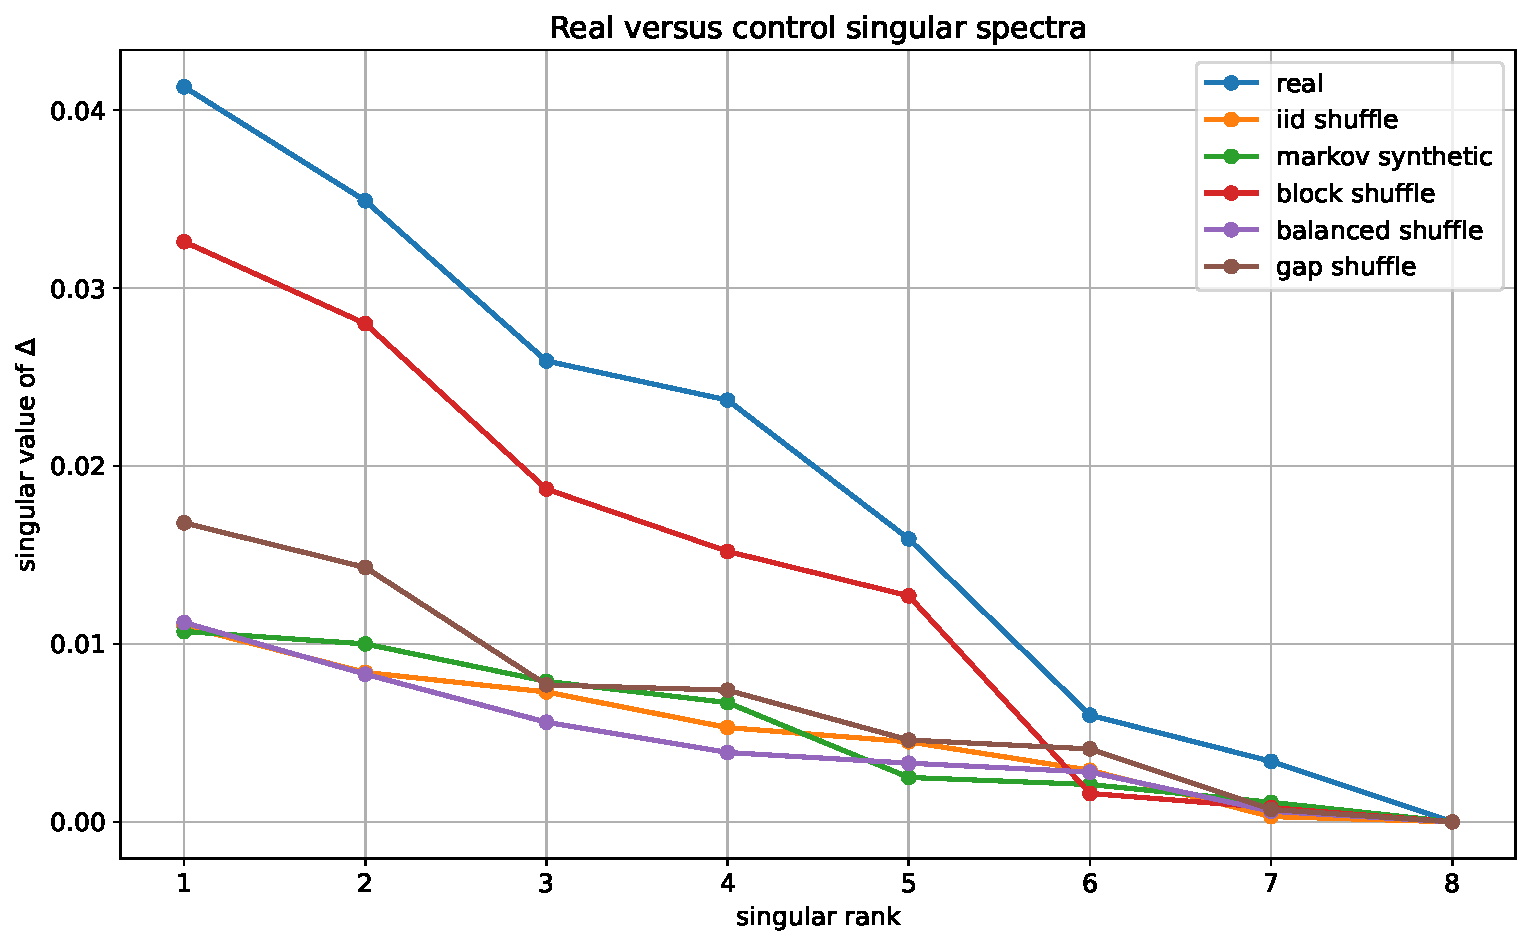
\includegraphics[width=0.92\linewidth]{figures/22_real_vs_control_singular_spectra.pdf}
\caption{Singular spectra of the two-step residual operator $\Delta=P^{(2)}_{\mathrm{emp}}-P^2$ for the real sequence and synthetic controls. The leading real singular modes exceed iid and Markov controls, indicating structured higher-order memory beyond first-order transition statistics.}
\label{fig:singular-spectra}
\end{figure}

\begin{figure}[htbp]
\centering
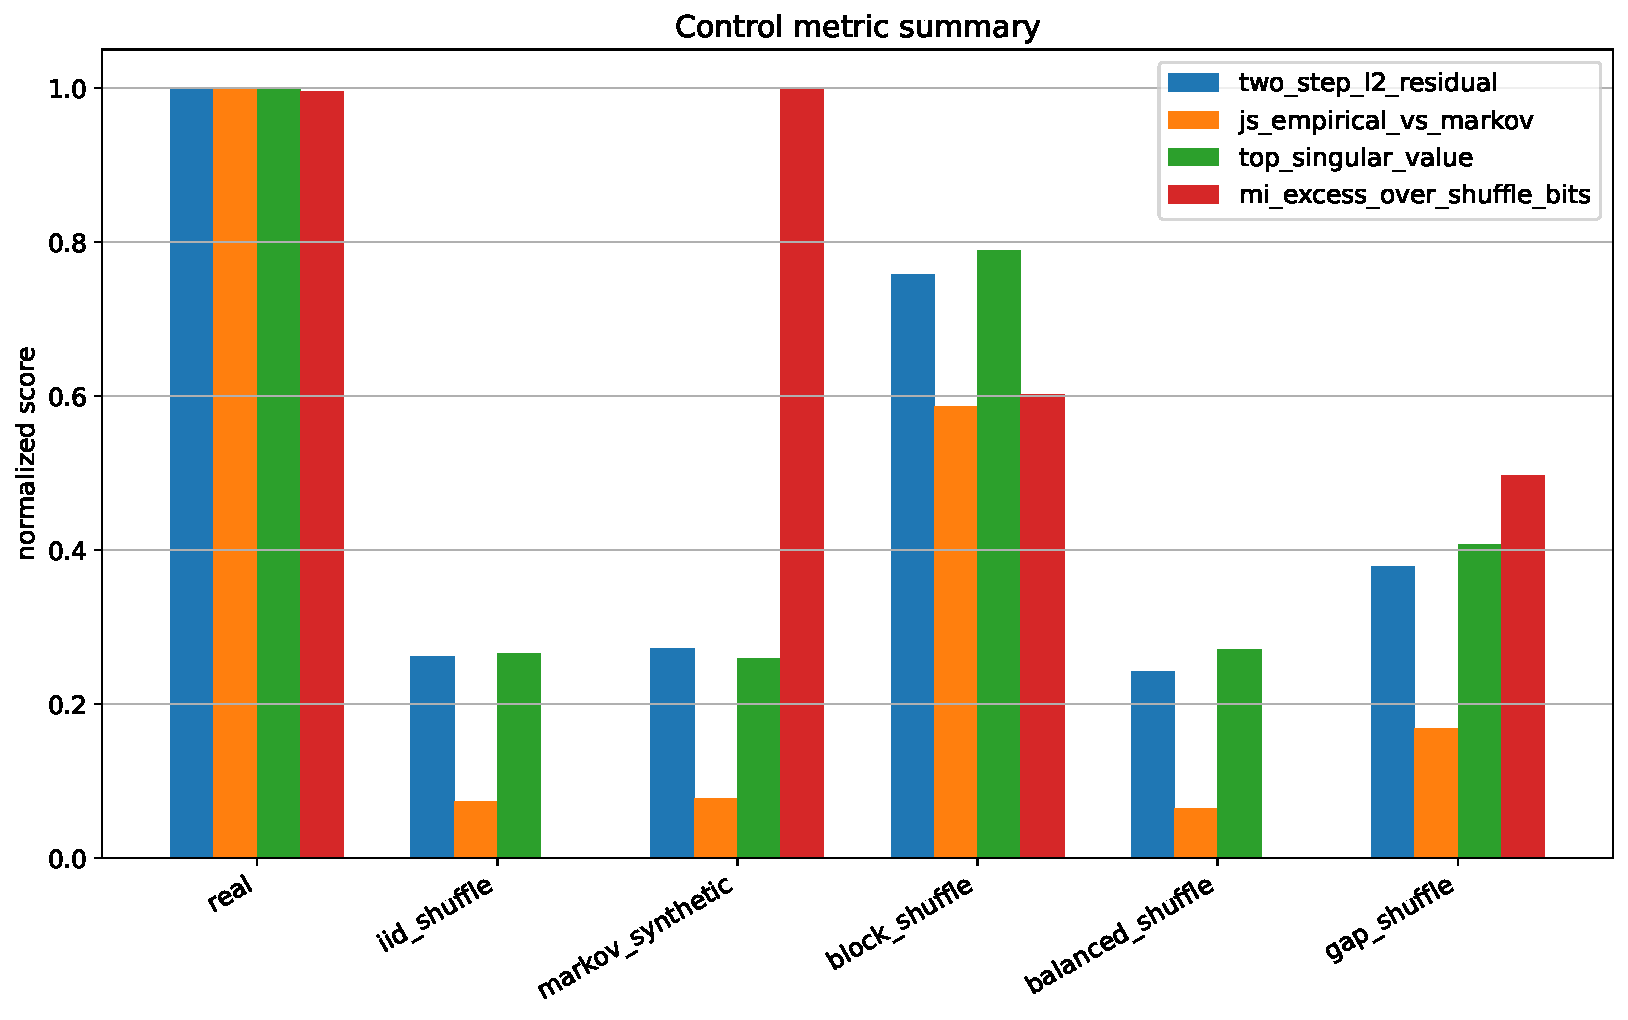
\includegraphics[width=0.92\linewidth]{figures/22_control_metric_summary.pdf}
\caption{Normalized comparison of the principal validation metrics across real and control sequences. The real sequence dominates two-step residual magnitude, JS distance, leading singular value, and mutual-information excess, while iid and balanced controls remain near the noise floor.}
\label{fig:control-summary}
\end{figure}

\begin{figure}[htbp]
\centering
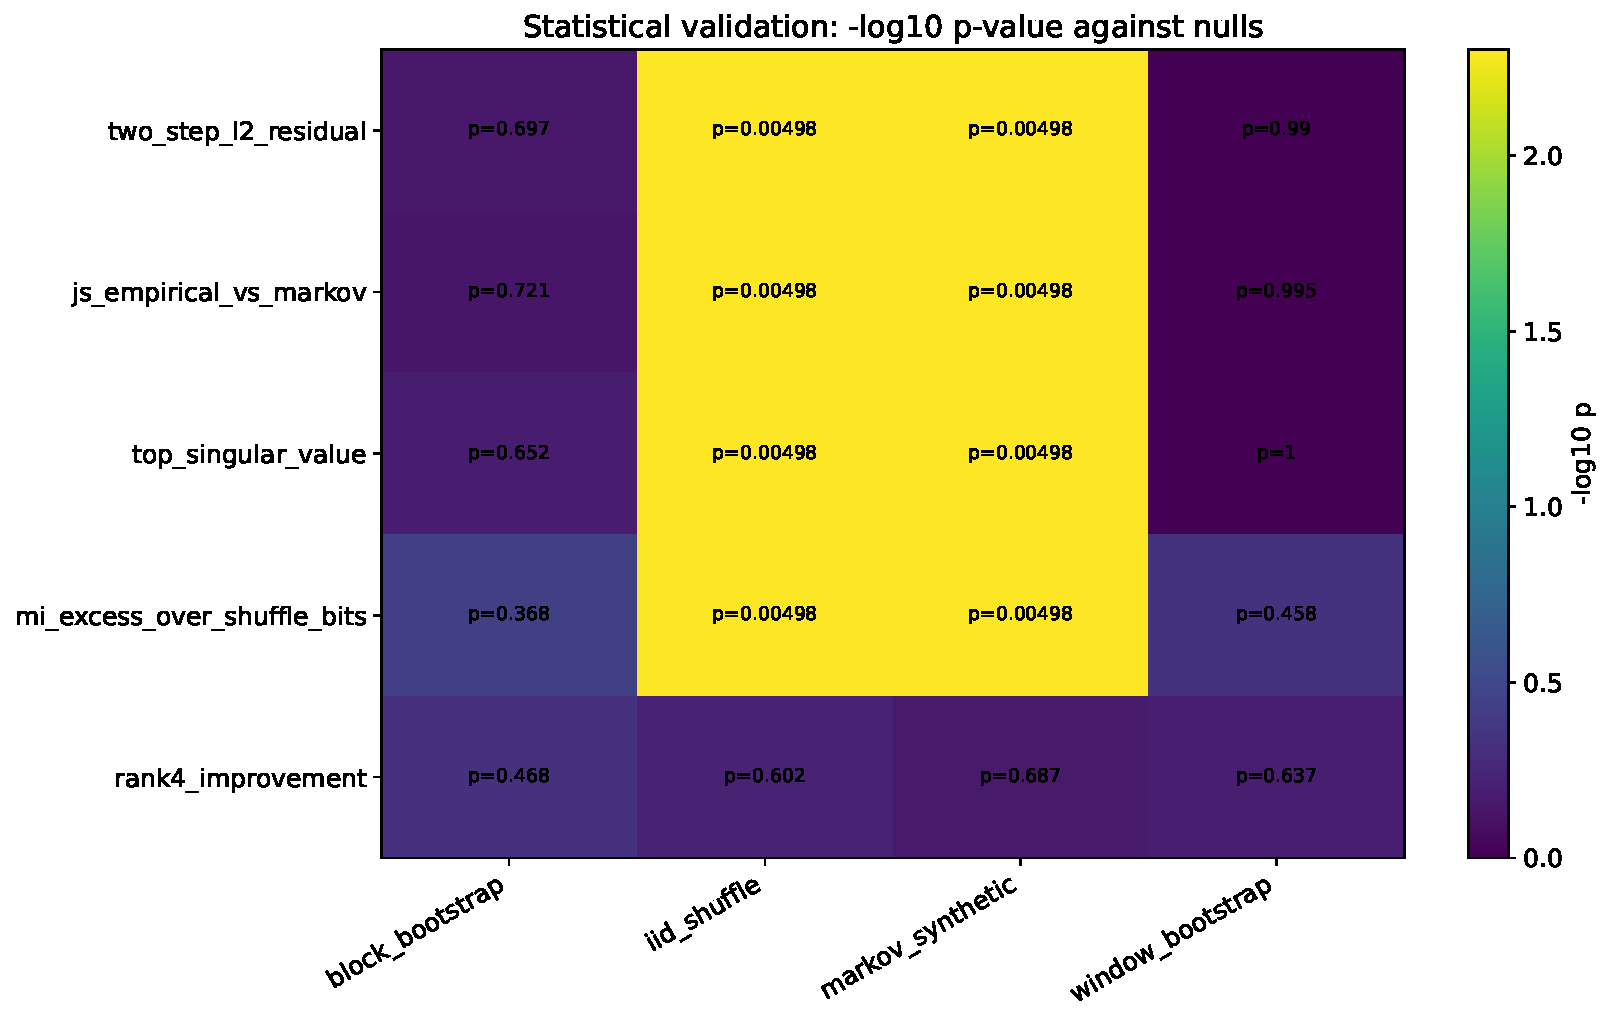
\includegraphics[width=0.92\linewidth]{figures/22_statistical_validation_pvalue_heatmap.pdf}
\caption{Permutation and resampling validation summarized as $-\log_{10}(p)$ values. Structure-destroying iid and Markov nulls reject multiple real-sequence metrics, while block and window resampling retain local structure and therefore behave as conservative controls.}
\label{fig:pvalue-heatmap}
\end{figure}

\begin{figure}[htbp]
\centering
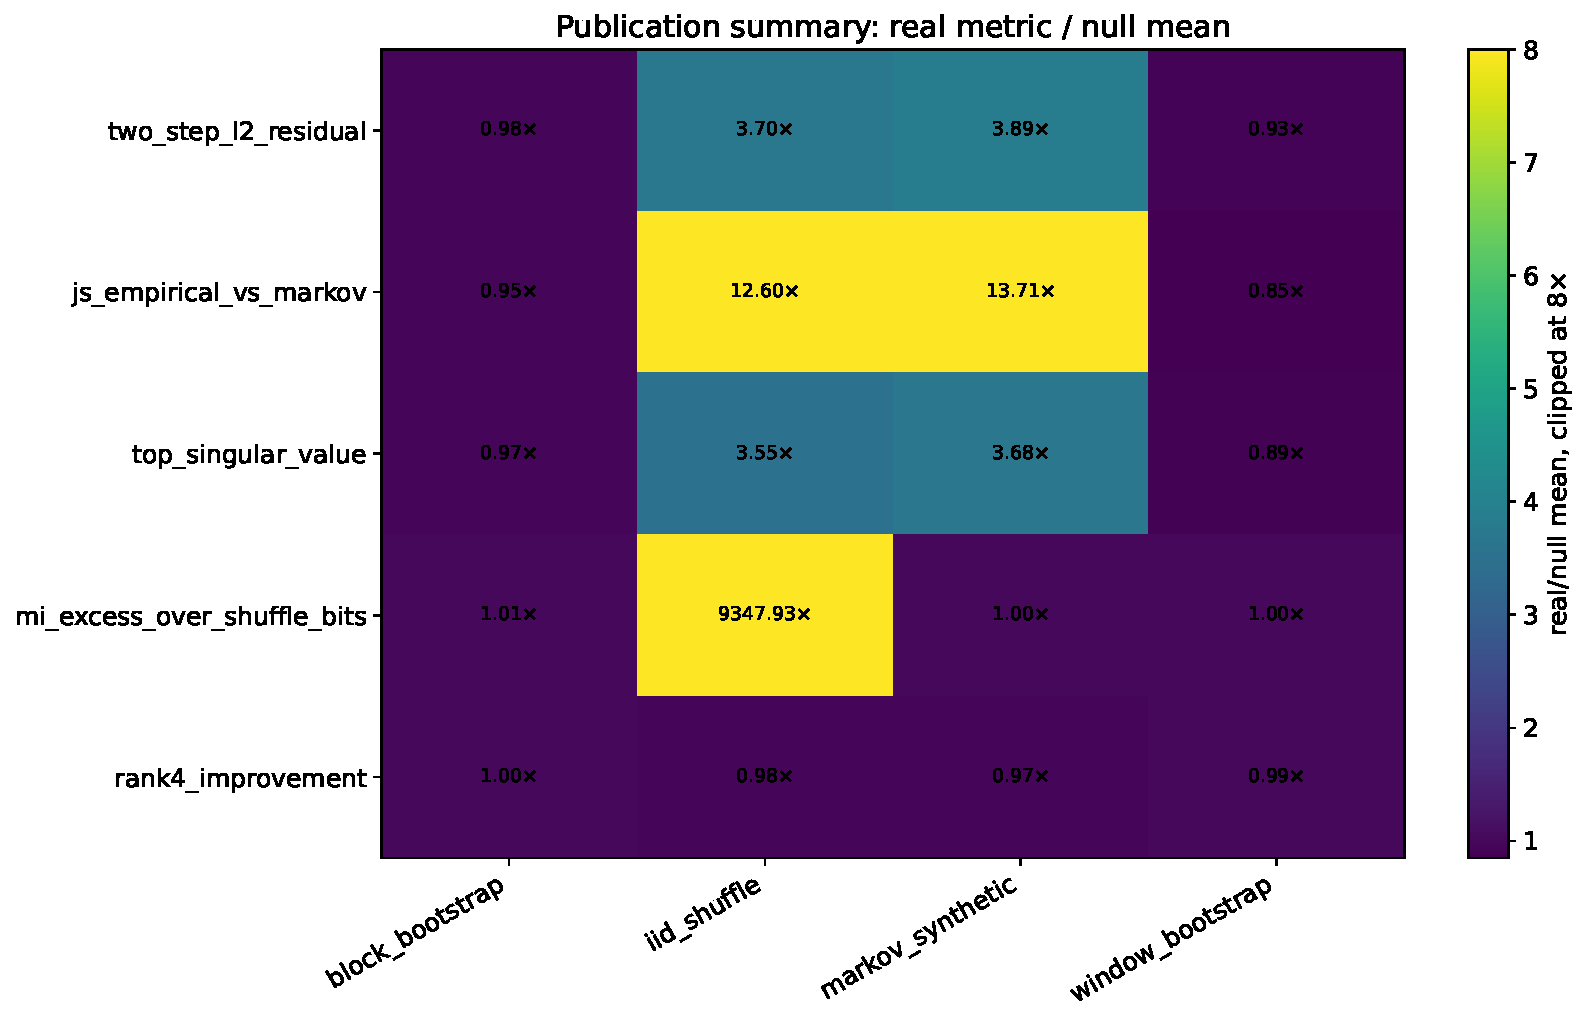
\includegraphics[width=0.92\linewidth]{figures/22_publication_summary_ratio_heatmap.pdf}
\caption{Effect-size summary showing real metrics divided by null means. Ratios above one indicate real-sequence excess relative to a null ensemble; clipped color scaling preserves readability while annotations retain numerical ratios.}
\label{fig:ratio-heatmap}
\end{figure}

\begin{figure}[htbp]
\centering
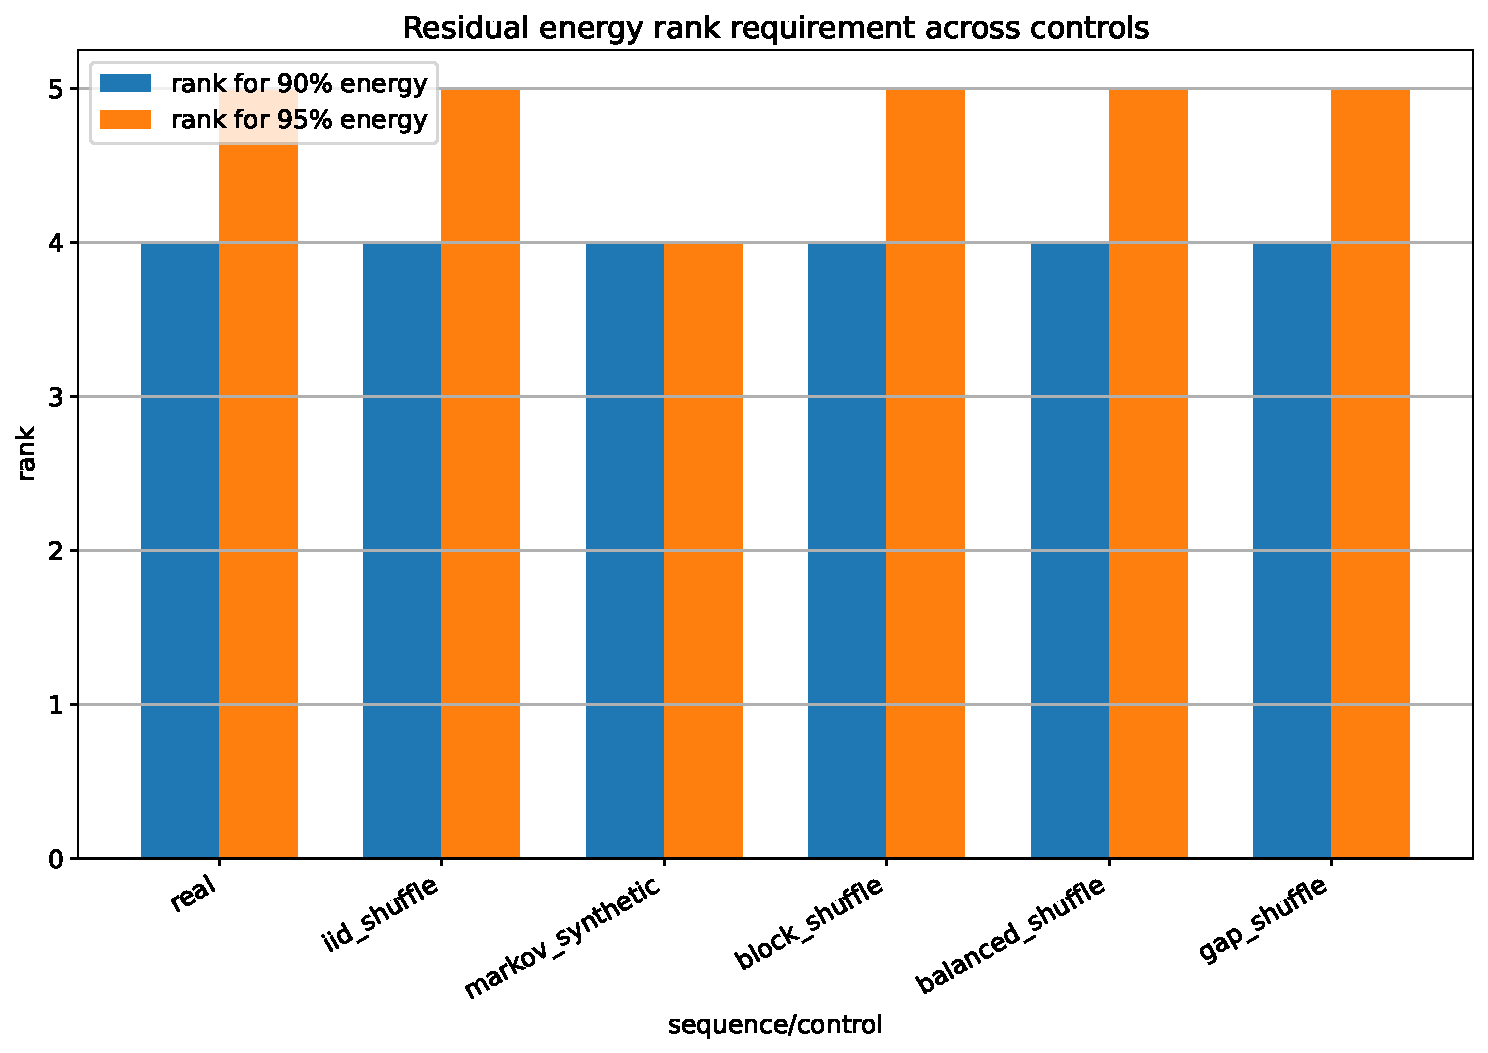
\includegraphics[width=0.92\linewidth]{figures/22_residual_energy_rank_requirement.pdf}
\caption{Low-rank energy summary for the residual operator. The real sequence remains concentrated in a small number of singular modes, supporting a compact memory correction rather than high-dimensional noise fitting.}
\label{fig:rank-requirement}
\end{figure}

\begin{figure}[htbp]
\centering
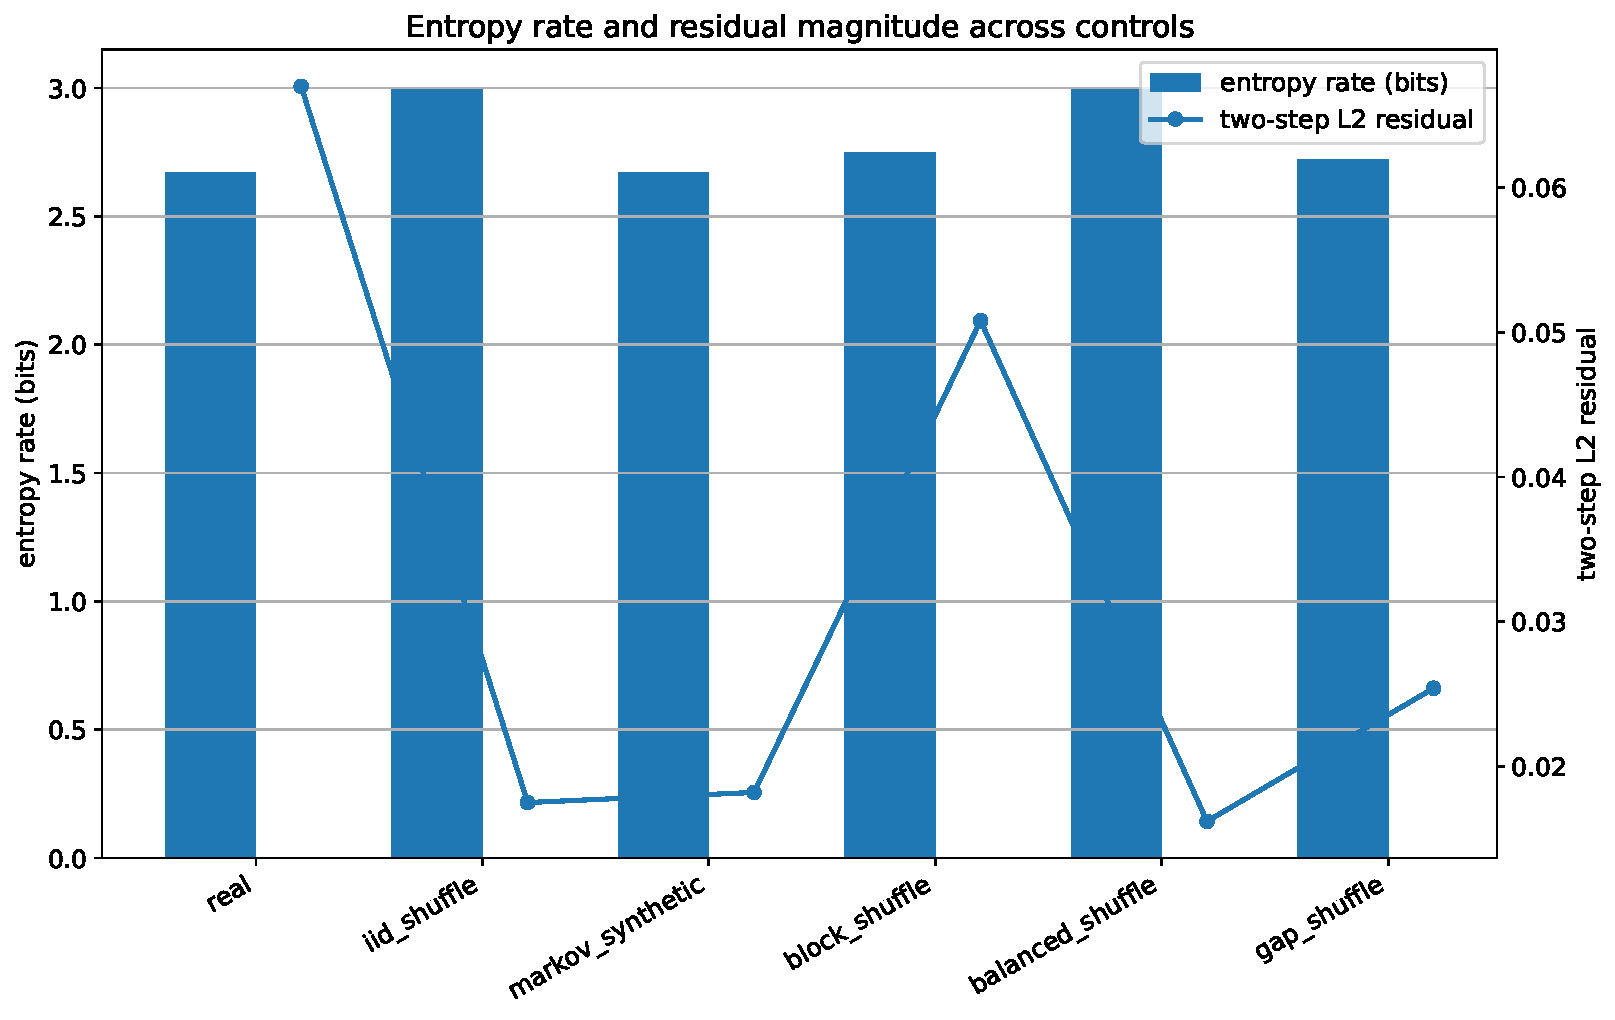
\includegraphics[width=0.92\linewidth]{figures/22_entropy_rate_and_residual_comparison.pdf}
\caption{Entropy and two-step residual magnitude across real and control sequences. Randomizing controls increase entropy and suppress residual memory, while the real sequence retains measurable structured deviation from the first-order Markov baseline.}
\label{fig:entropy-residual}
\end{figure}
